\subsection{Ridge Regression}

Now we applied the Ridge Regression to perform variable selection. In \Fig~\ref{fig:RidgeCoefVsLambda} is shown the coefficients' behavior as $\lambda$ increases. 

\begin{figure}[h]
	\centering
	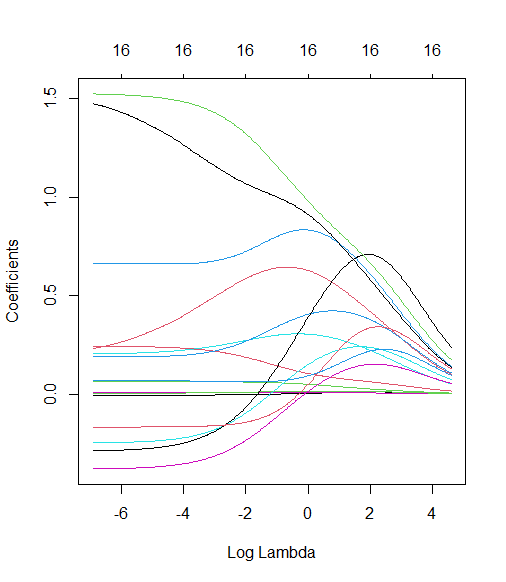
\includegraphics[width=0.4\linewidth]{ImageFiles/Regression/Ridge/RidgeCoefVsLambda}
	\caption{Ridge Regression coefficients as function of $\lambda$.}
	\label{fig:RidgeCoefVsLambda}
\end{figure}

It is possible to observe that for enough large values of $\lambda$, around $10^2$, all the coefficients tend to become close to zero. However, they are never exactly zero.

To select the optimal value of the penalization factor $\lambda$ we employed ``k-Fold Cross-Validation'' with $k=10$. In \Fig~\ref{fig:RidgeCvPlot} it is possible to observe the trend of the cross-validated MSE (``\textit{Mean Square Error}'') when $\lambda$ increases. The optimal value was found to be $\lambda_{opt} = 0.0304$.

\begin{figure}[h]
	\centering
	\begin{subfigure}{.6\textwidth}
		\centering
		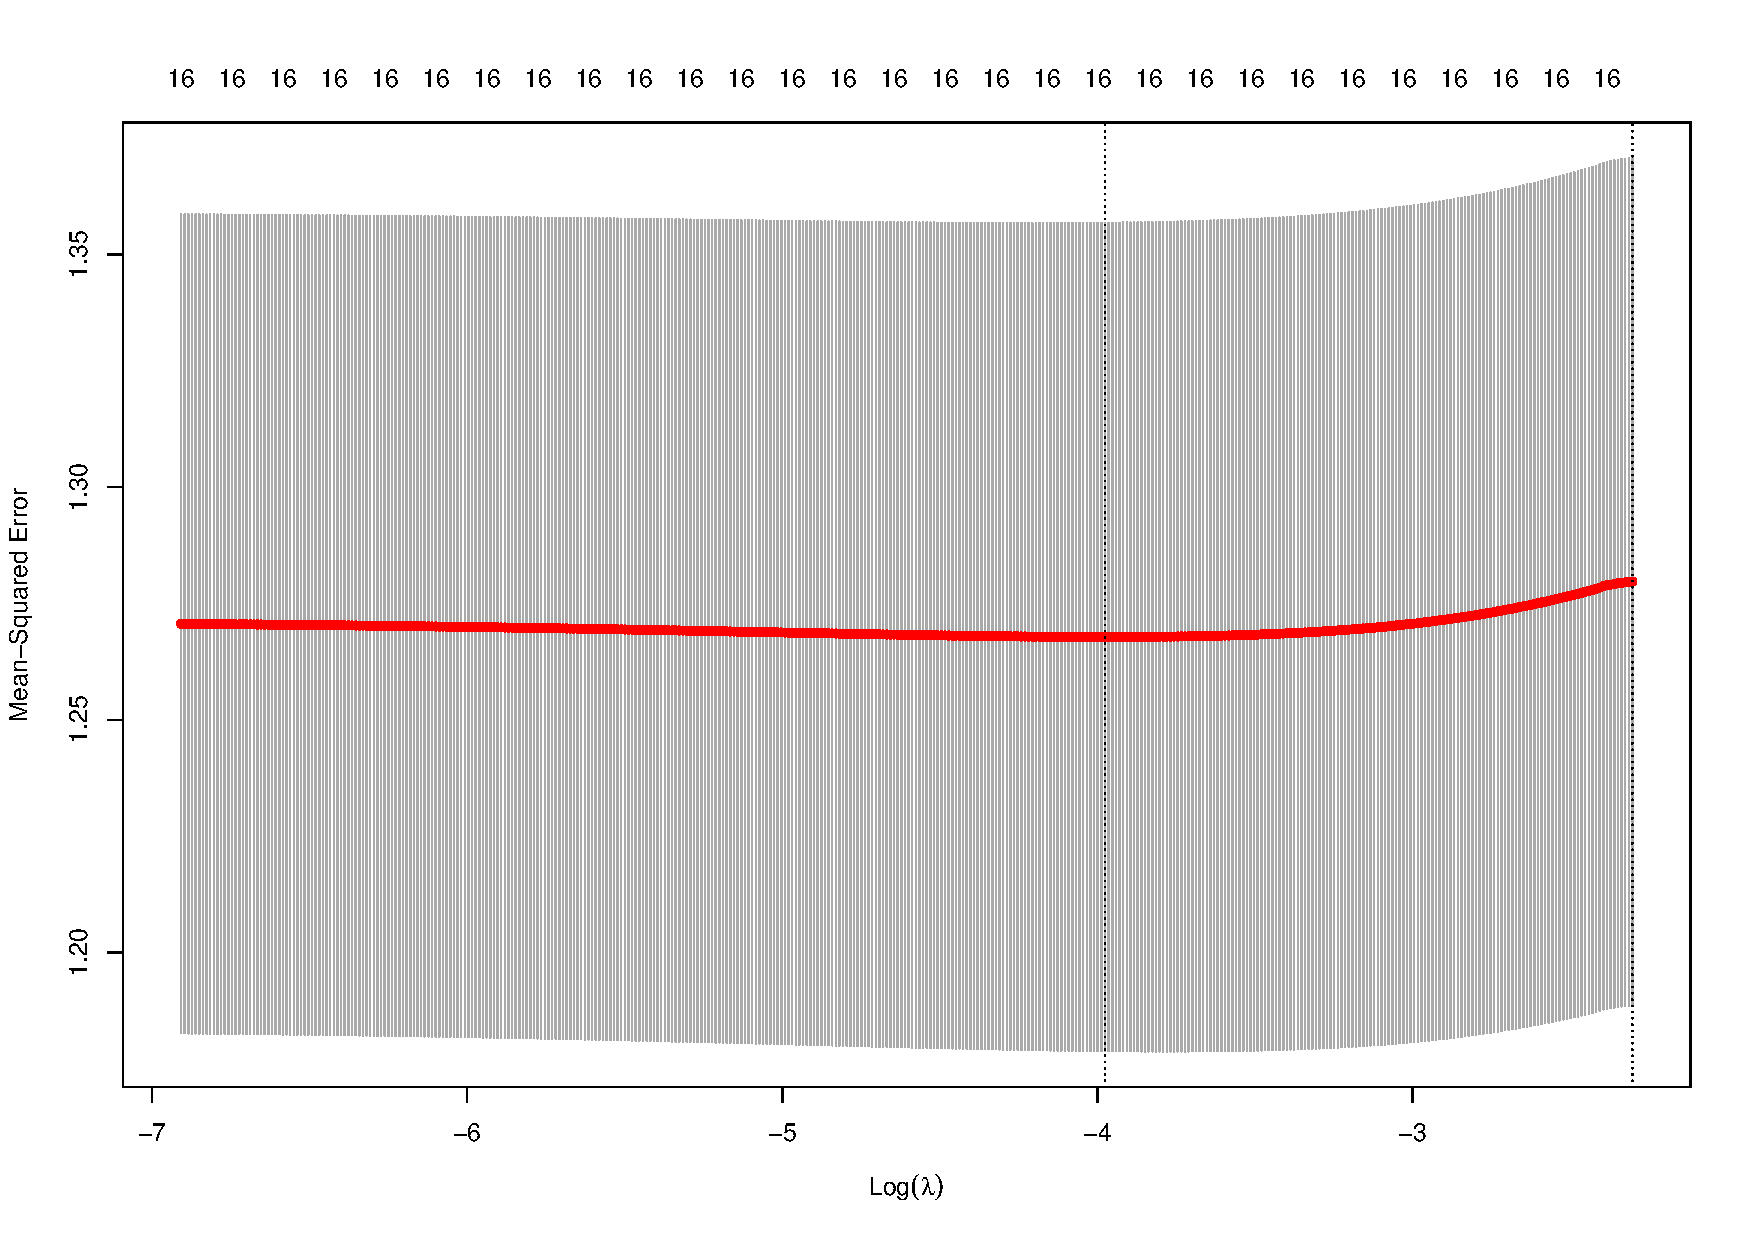
\includegraphics[width=0.7\linewidth]{ImageFiles/Regression/Ridge/RidgeCvPlot}
		\caption{Ridge cross validated MSE as function of $\lambda$.}
		\label{fig:RidgeCvPlot}
	\end{subfigure}%
	\begin{subfigure}{.6\textwidth}
		\centering
		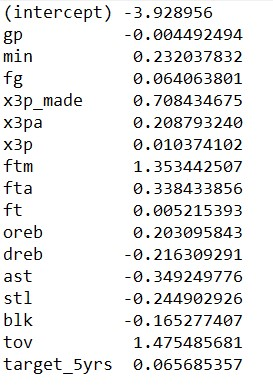
\includegraphics[width=0.4\linewidth]{ImageFiles/Regression/Ridge/FinalRidgeCoef}
		\caption{Ridge Regression coefficients with $\lambda_{opt}$.}
		\label{fig:FinalRidgeCoef}
	\end{subfigure}
	\caption{Ridge Regression model.}
	\label{fig:FinalRidgeModel}
\end{figure}

We fit the final model using the optimal $\lambda$ value ($\lambda_{opt}$). The resulting coefficients are displayed in Figure~\ref{fig:FinalRidgeCoef}. For this model we computed also the test MSE and it is $MSE_{test} = 1.33$

In this case the Ridge Penalization does not reduce the number of coefficients, and it does not even improve significantly the MSE. We then can conclude that using Ridge Regression is not useful for our purposes.
